\documentclass[pdftex,a4paper,12pt,twocolumn,fleqn,captions=tableheading]{scrartcl}

\usepackage[british]{babel}
\usepackage[utf8]{inputenc}
\usepackage[T1]{fontenc}
\usepackage{graphicx}
\usepackage{booktabs}
\usepackage{caption}
\usepackage{subcaption}
\usepackage{lmodern}
\usepackage{microtype}
\usepackage{textcomp}
\usepackage{amssymb}
\usepackage{epstopdf}
\usepackage{capt-of}
\usepackage{amsmath}
\usepackage{float}
\usepackage{xfrac}
\usepackage{dblfloatfix}
\usepackage{url}
\usepackage[squaren,Gray]{SIunits}
\usepackage{commath}
\usepackage{listings}
% \usepackage{siunitx}

\addtokomafont{caption}{\small}
\setkomafont{captionlabel}{\sffamily\bfseries}

\usepackage[nottoc]{tocbibind}

% page layout
\usepackage[a4paper,onecolumn]{geometry}
\geometry{hmargin=60pt,top=60pt,bottom=80pt}
% \geometry{onecolumn,columnsep=20pt}
\geometry{head=10pt,headsep=20pt,foot=35pt}

% header and footer
\usepackage{fancyhdr}
\setlength{\headheight}{15pt}
\pagestyle{fancy}
%\fancyheadoffset{9pt}
%\fancyfootoffset{9pt}
\lhead{}	\chead{IMU yellow boxes}	\rhead{}
\lfoot{}	\cfoot{J. Rabault \\ \thepage}	\rfoot{}
%\renewcommand{\headrulewidth}{0,1 mm}
\renewcommand{\footrulewidth}{\headrulewidth}

\begin{document}
% top matter
\title{Details about the IMU yellow boxes}
\author{J. Rabault
  }
\date{\today}

\maketitle

\section{Introduction}

This is an addition to the main manual (see the "User Manual" on this repo), with specific images / tips and tricks about the yellow IMU boxes. \\

Content of the shipment:

\begin{itemize}
  \item 2 yellow pelican cases containing the IMU logger, battery, and electronics
  \item 1 charger with 2 USB cables for charging the batteries
  \item 2 SD card adapters (1 USB and 1 SD to micro SD).
\end{itemize}

\section{Some key elements}

Highlight of a few key elements of the logger follows in the pictures under.

  \begin{figure}
  \begin{center}
  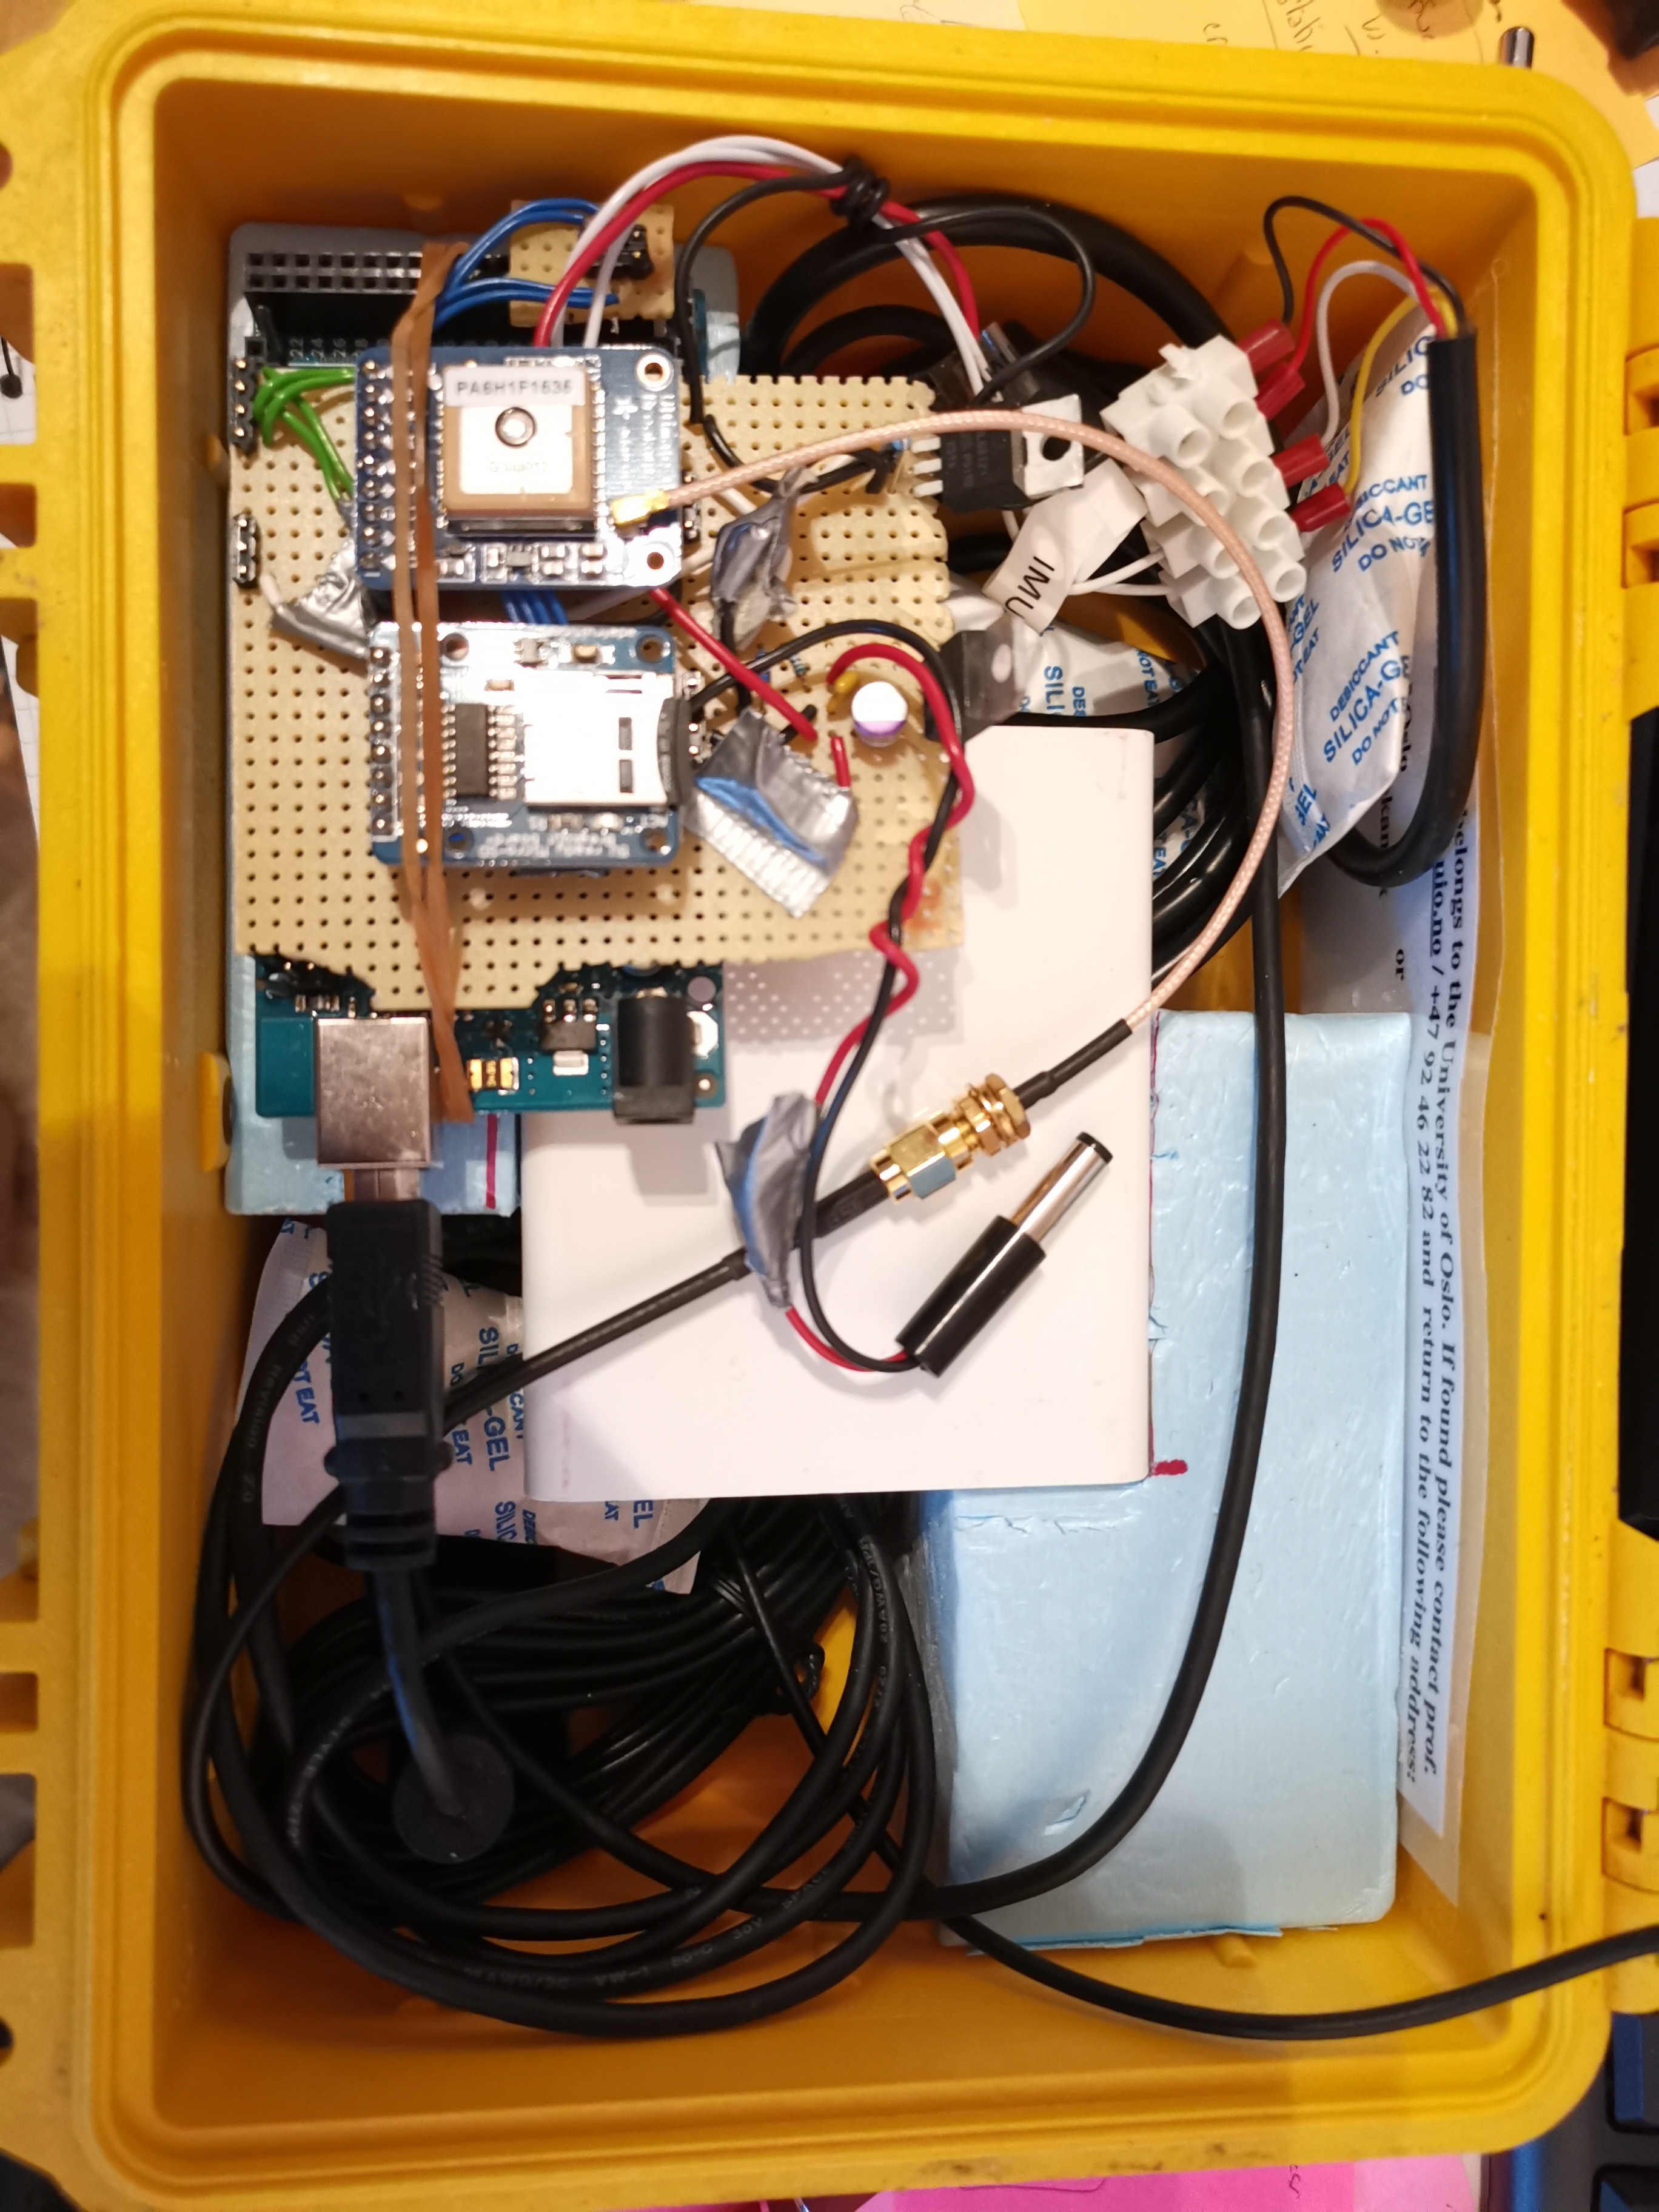
\includegraphics[width=.8\textwidth]{Figures/general_overview}
  \caption{General overview of the setup of the "yellow loggers". Note that the USB cable is usually disconnected from the Arduino board under transport (end that has a "square USB" connector), so remember to instert it before trying to turn the instrument on. On this picture, the USB cable is inserted into the Arduino.}
  \end{center}
  \end{figure}

  \begin{figure}
  \begin{center}
  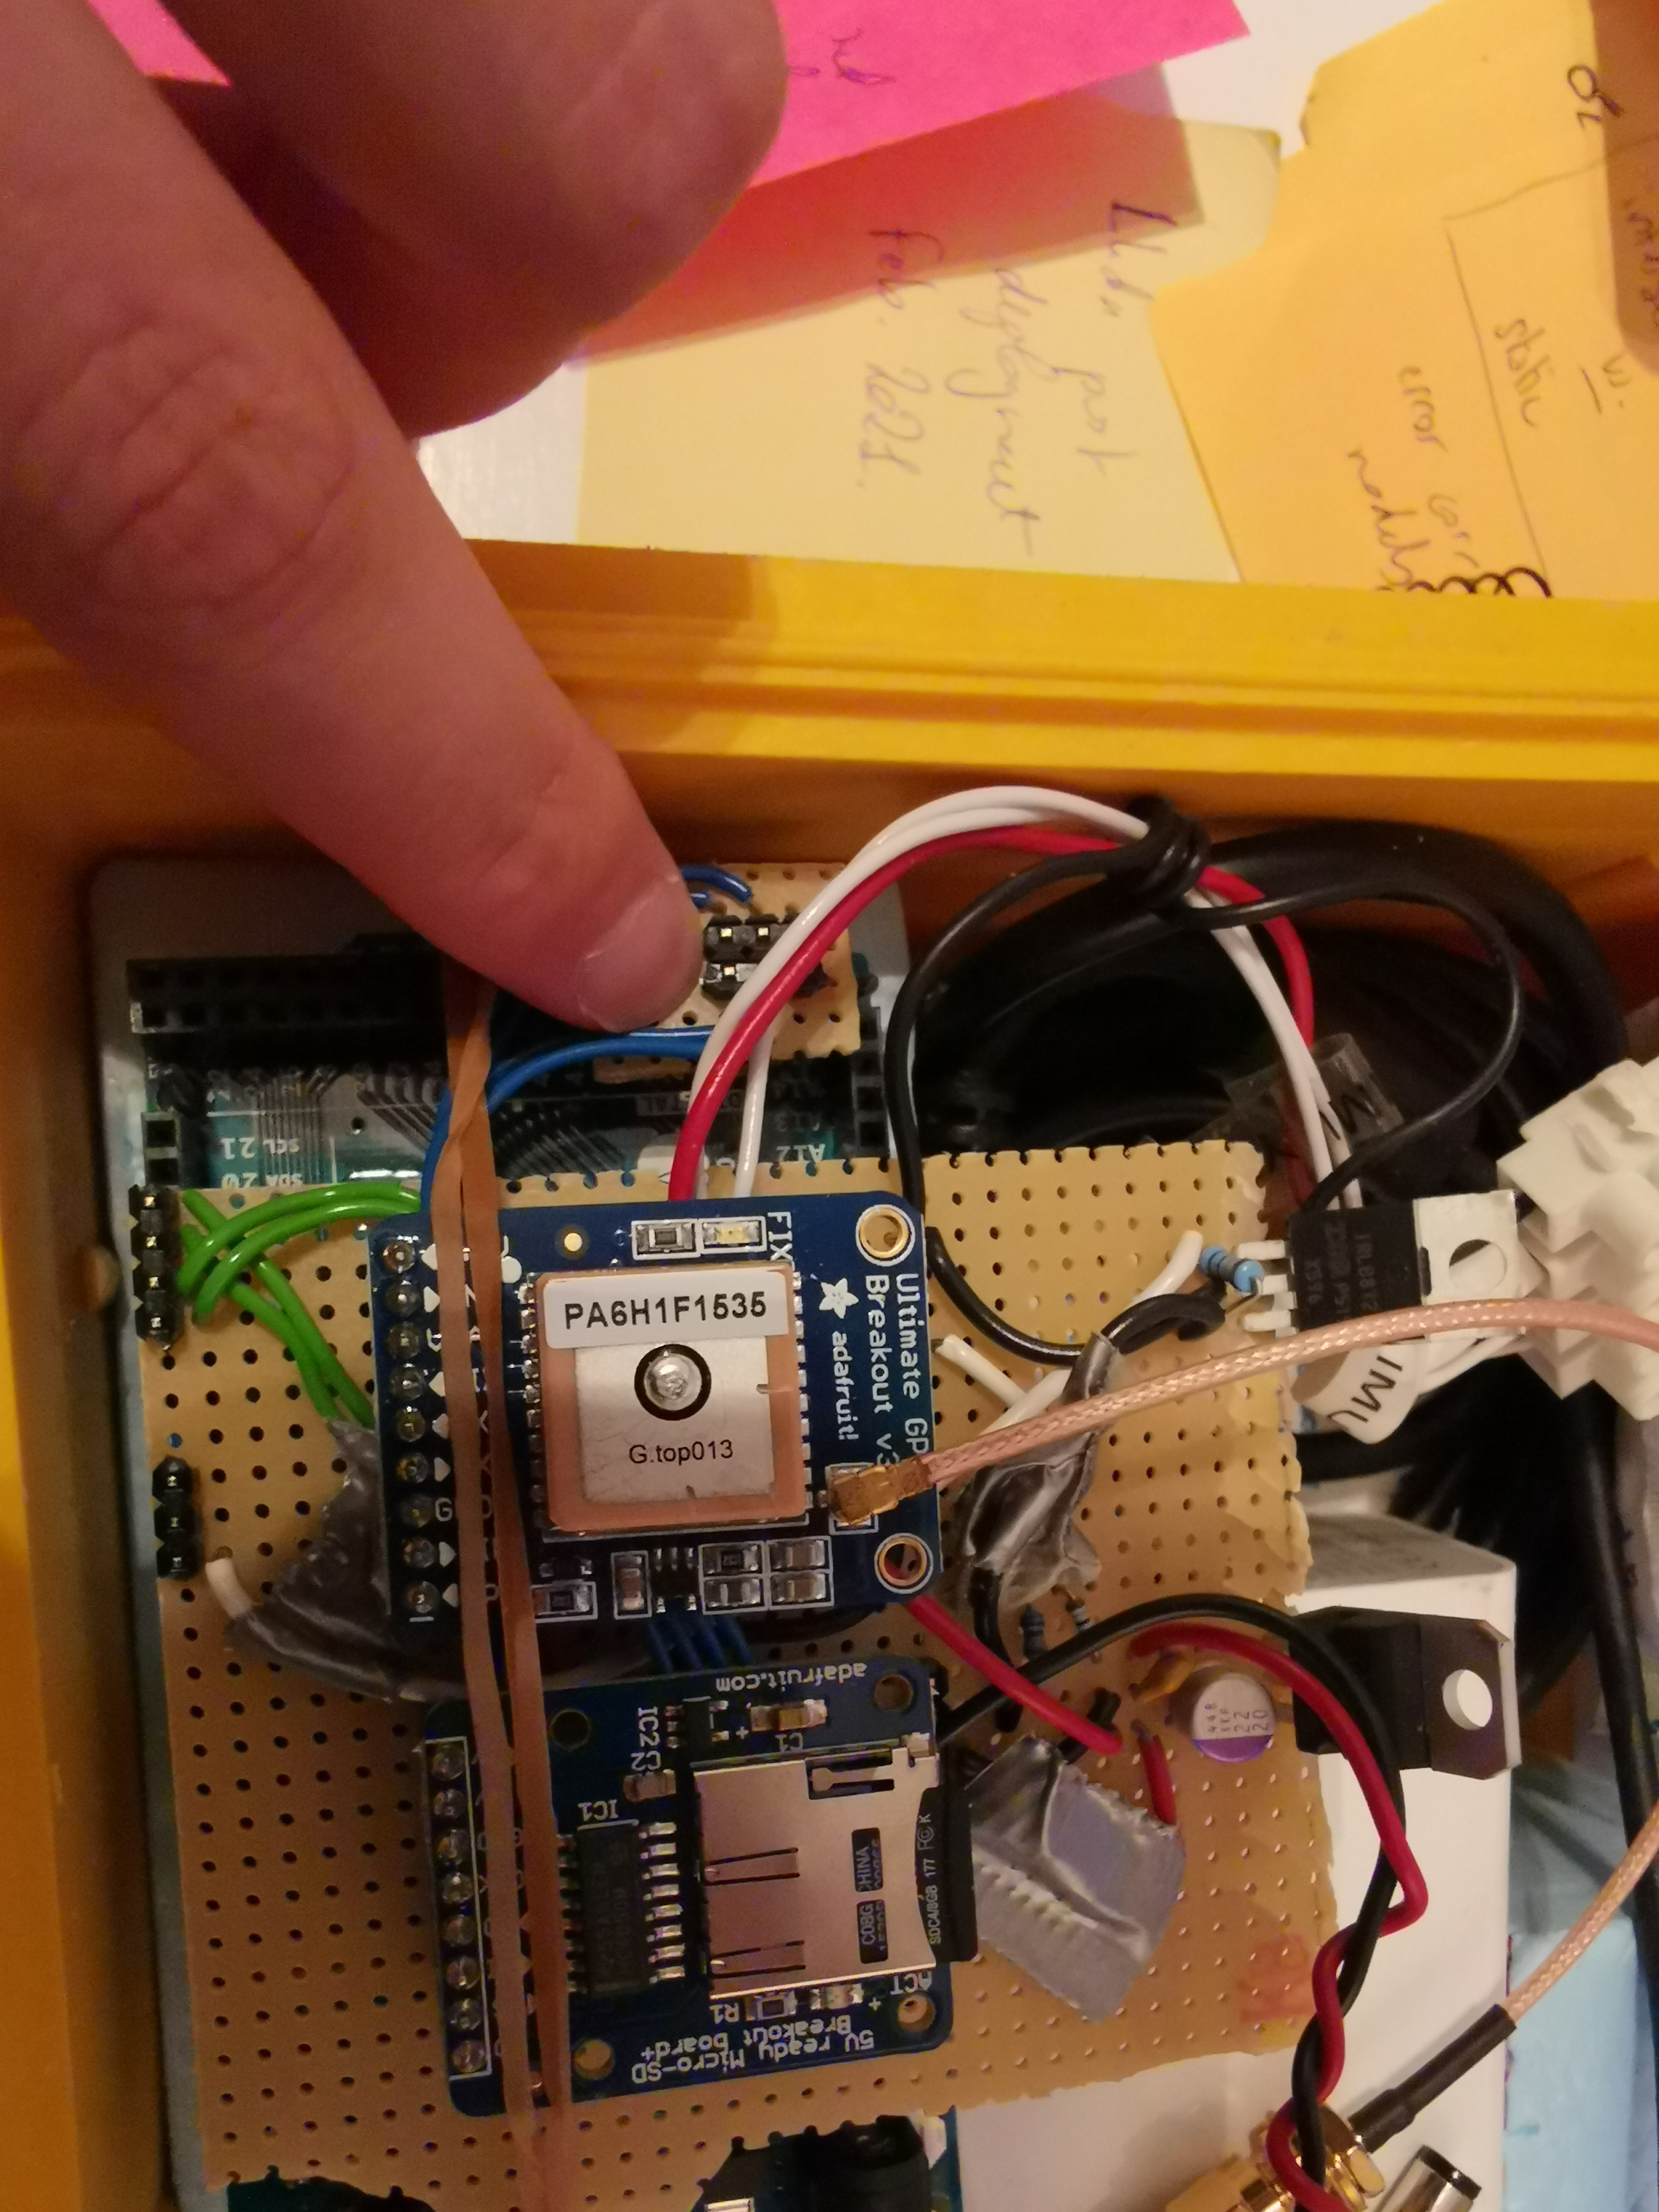
\includegraphics[width=.8\textwidth]{Figures/side_pcb}
  \caption{The "side PCB". In case of very heavy vibrations during transport it may pop out. If so, put it back in place. It can be a good idea to slightly press it in position by pushing slightly on it with the finger before deployment. Note the orientation: the 2 non connected pins go to the 2 most outwards slots of the underlying header.}
  \end{center}
  \end{figure}
  
  \begin{figure}
  \begin{center}
  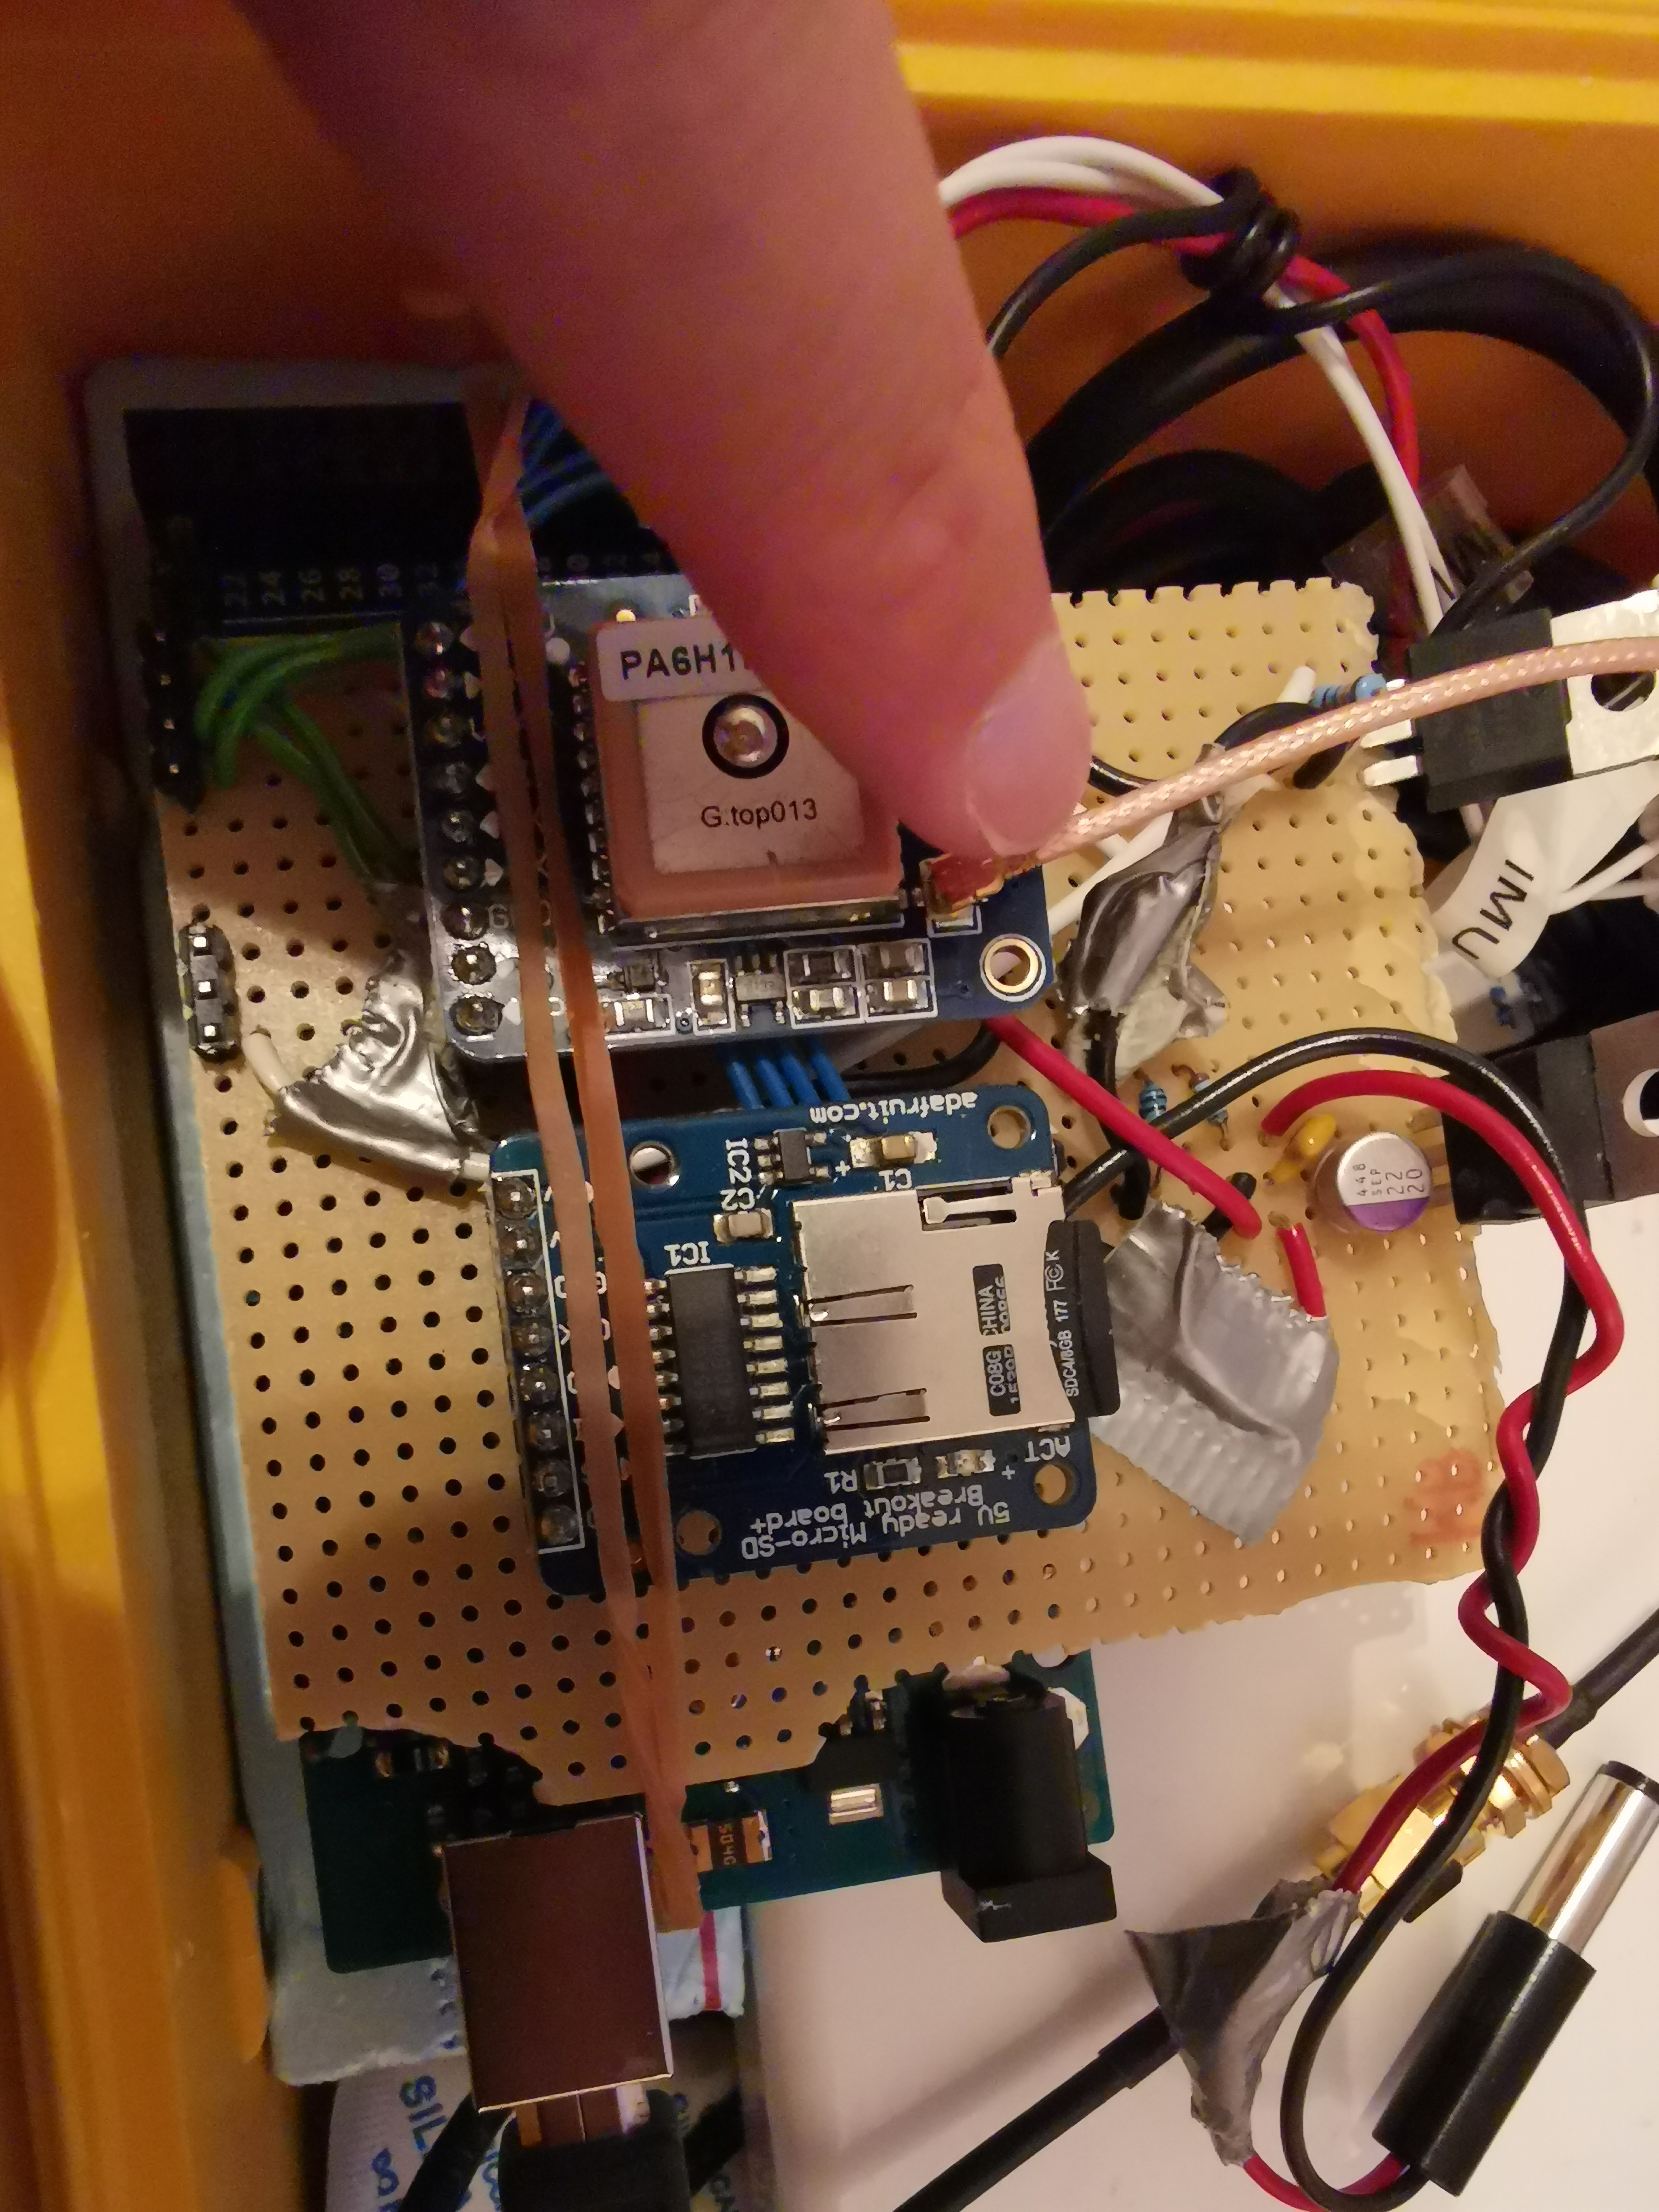
\includegraphics[width=.8\textwidth]{Figures/gps_connector}
  \caption{The GPS connector. This is a relatively sensitive connector that may pop out in case of heavy vibration. It can be a good idea to check that it is well inserted by slightly pinching it (from its top and the bottom of the breakout) to make sure it is well engaged, before deployment.}
  \end{center}
  \end{figure}

  \begin{figure}
  \begin{center}
  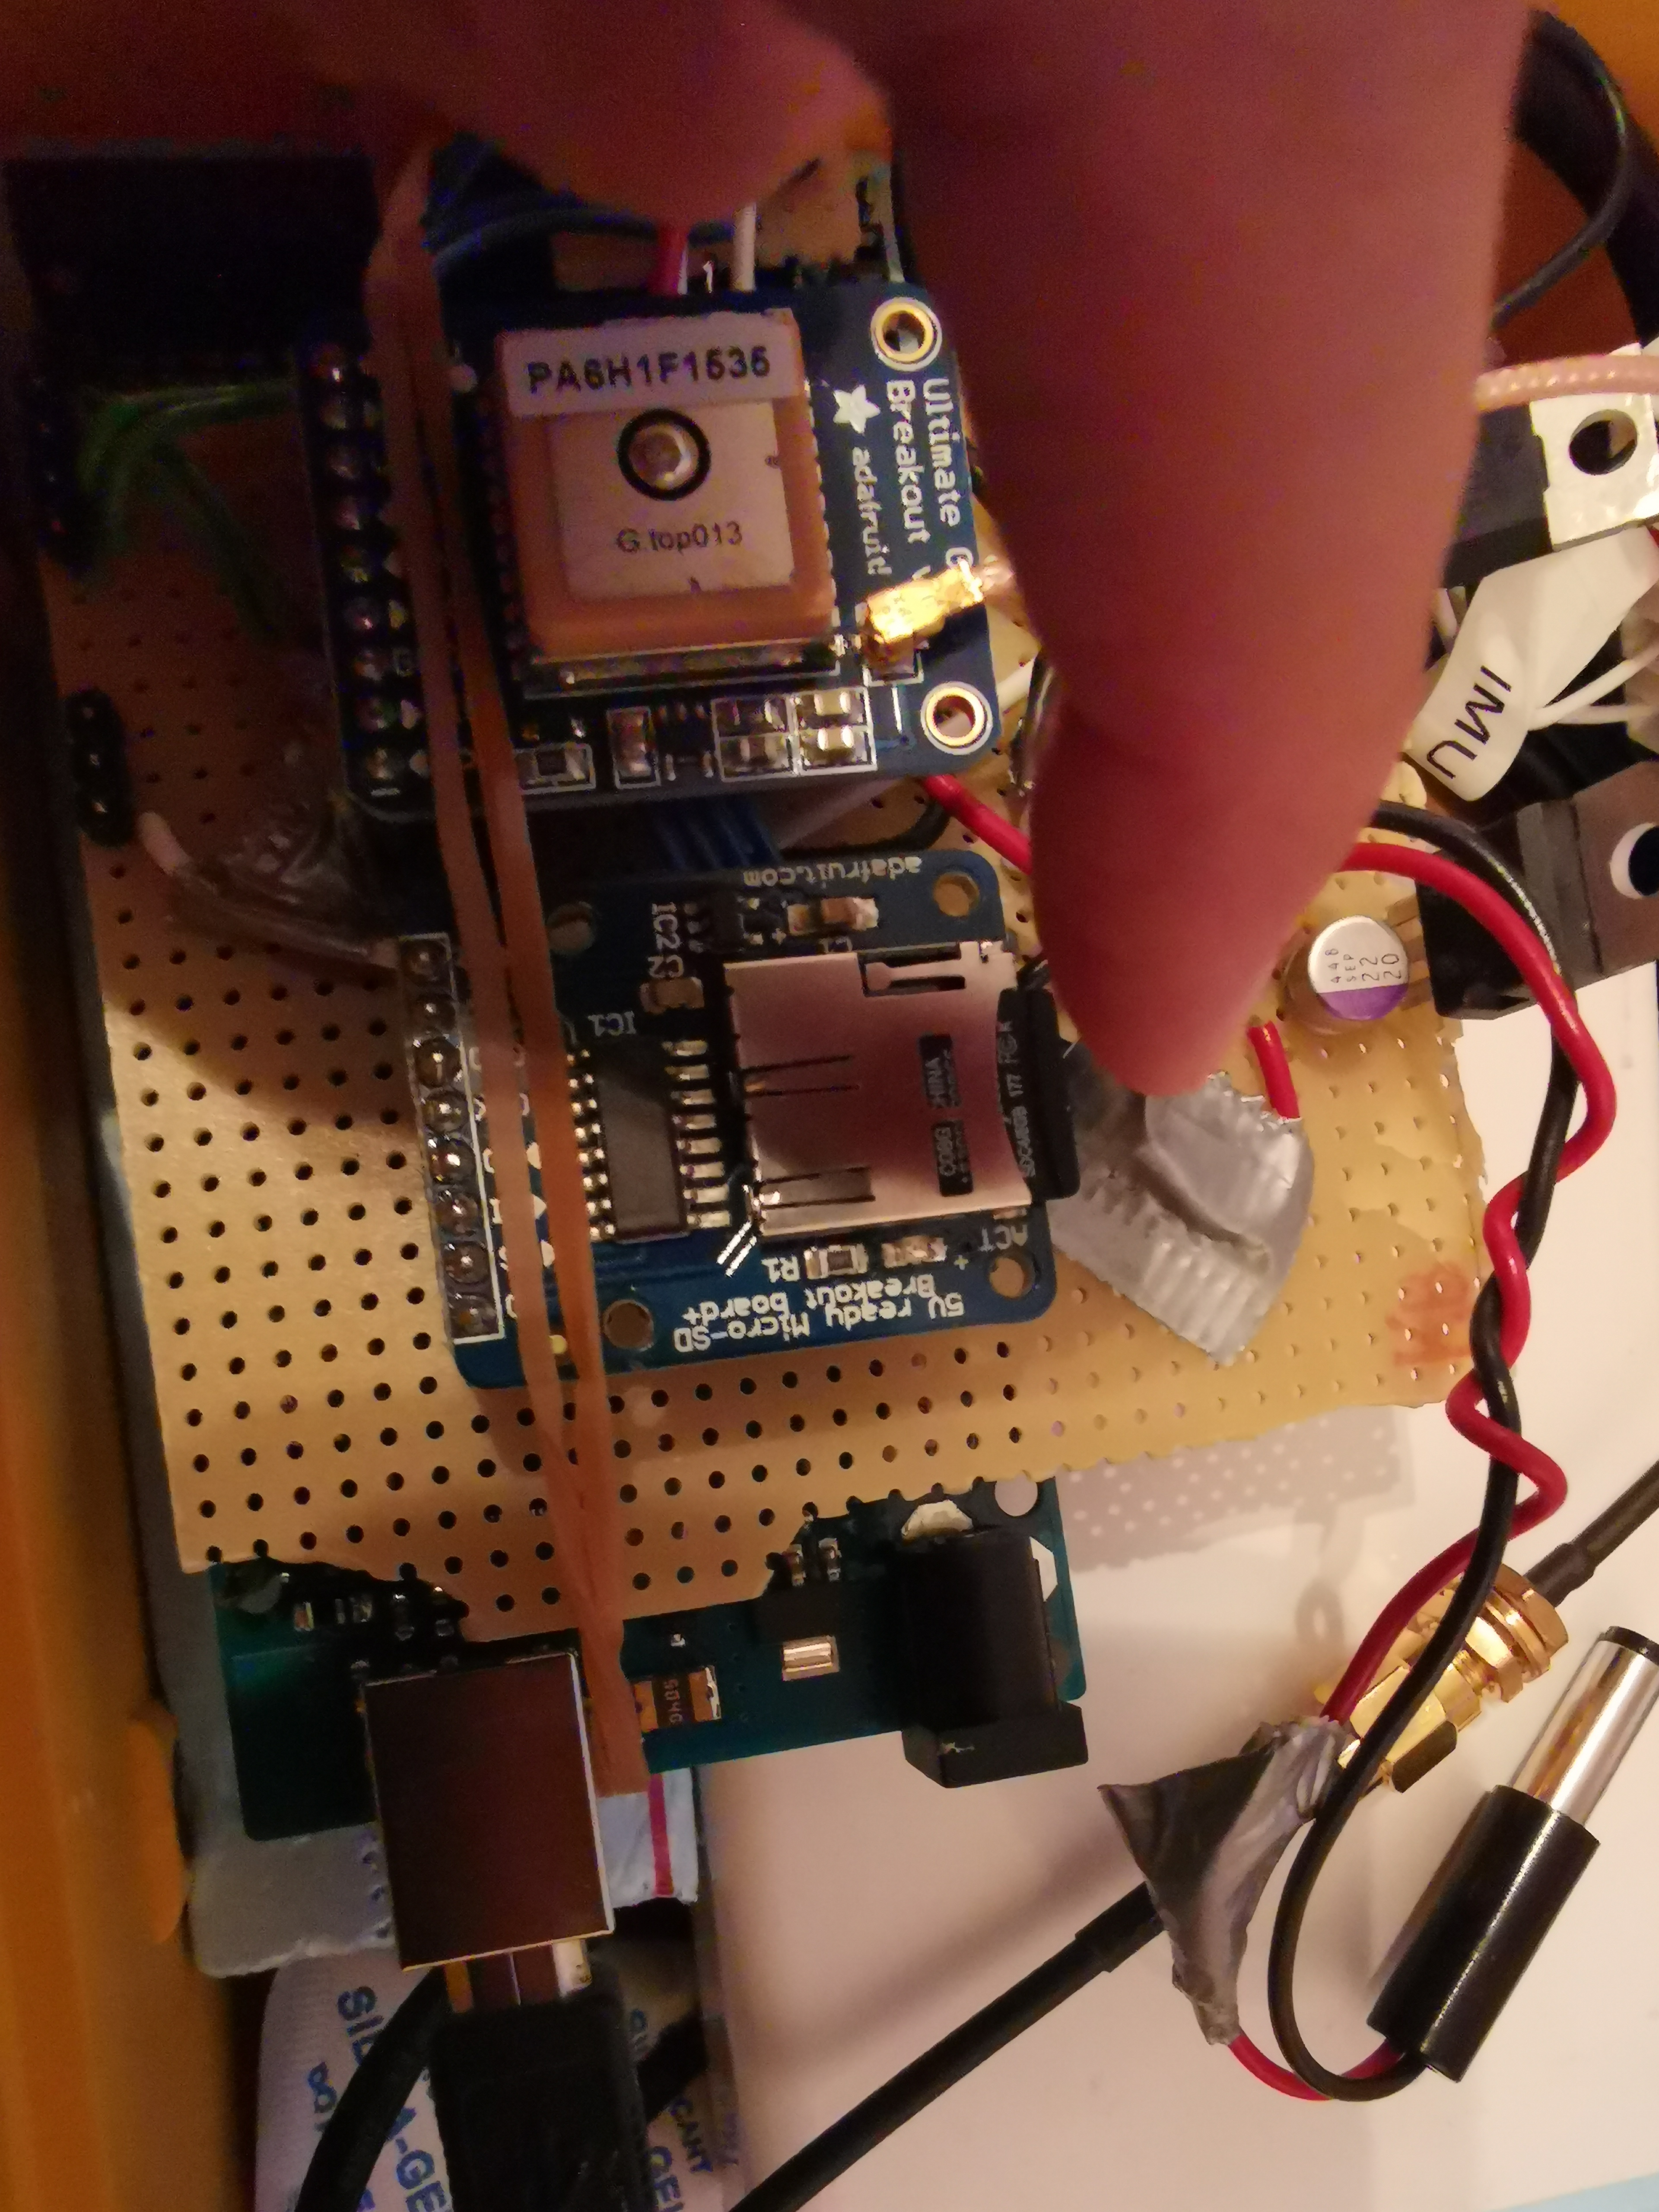
\includegraphics[width=.8\textwidth]{Figures/sd_card_slot}
  \caption{The SD card in its slot. This is a "push to insert / push to remove" slot, with a small spring in it. Make sure to correctly insert the SD card.}
  \end{center}
  \end{figure}

  \begin{figure}
  \begin{center}
  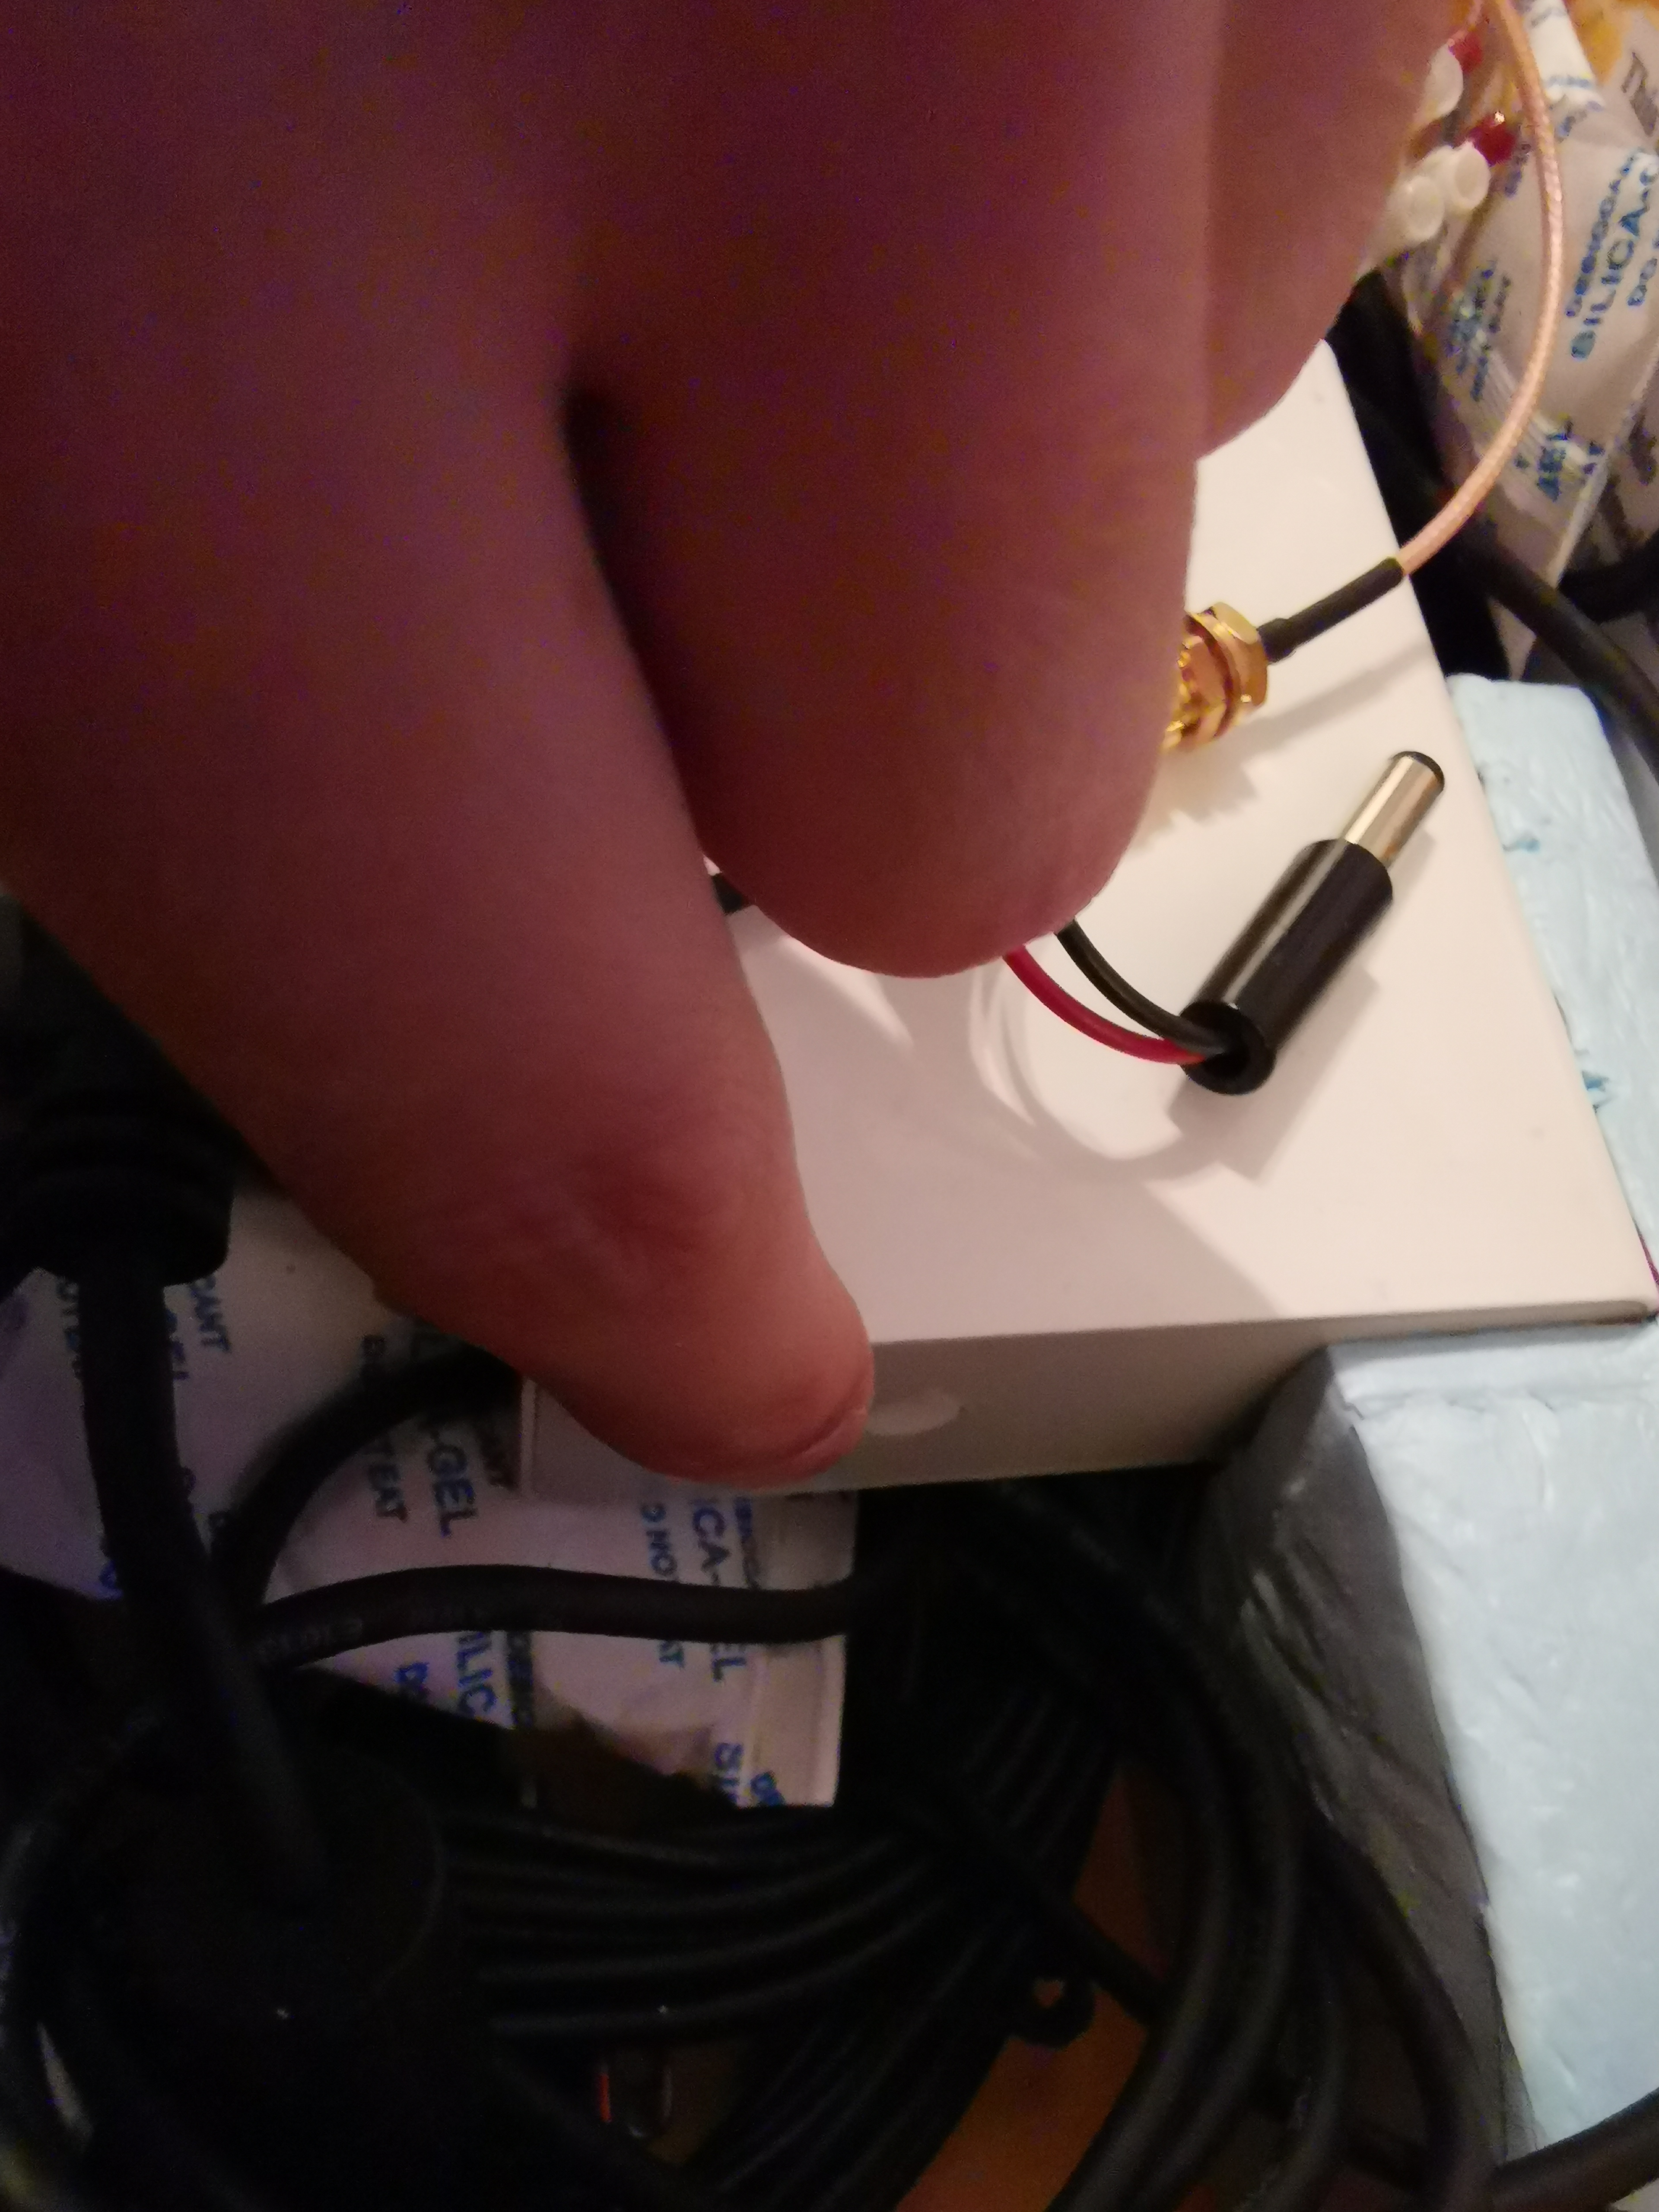
\includegraphics[width=.8\textwidth]{Figures/battery_on_off}
  \caption{The battery has on on / off button.}
  \end{center}
  \end{figure}
  
  \begin{figure}
  \begin{center}
  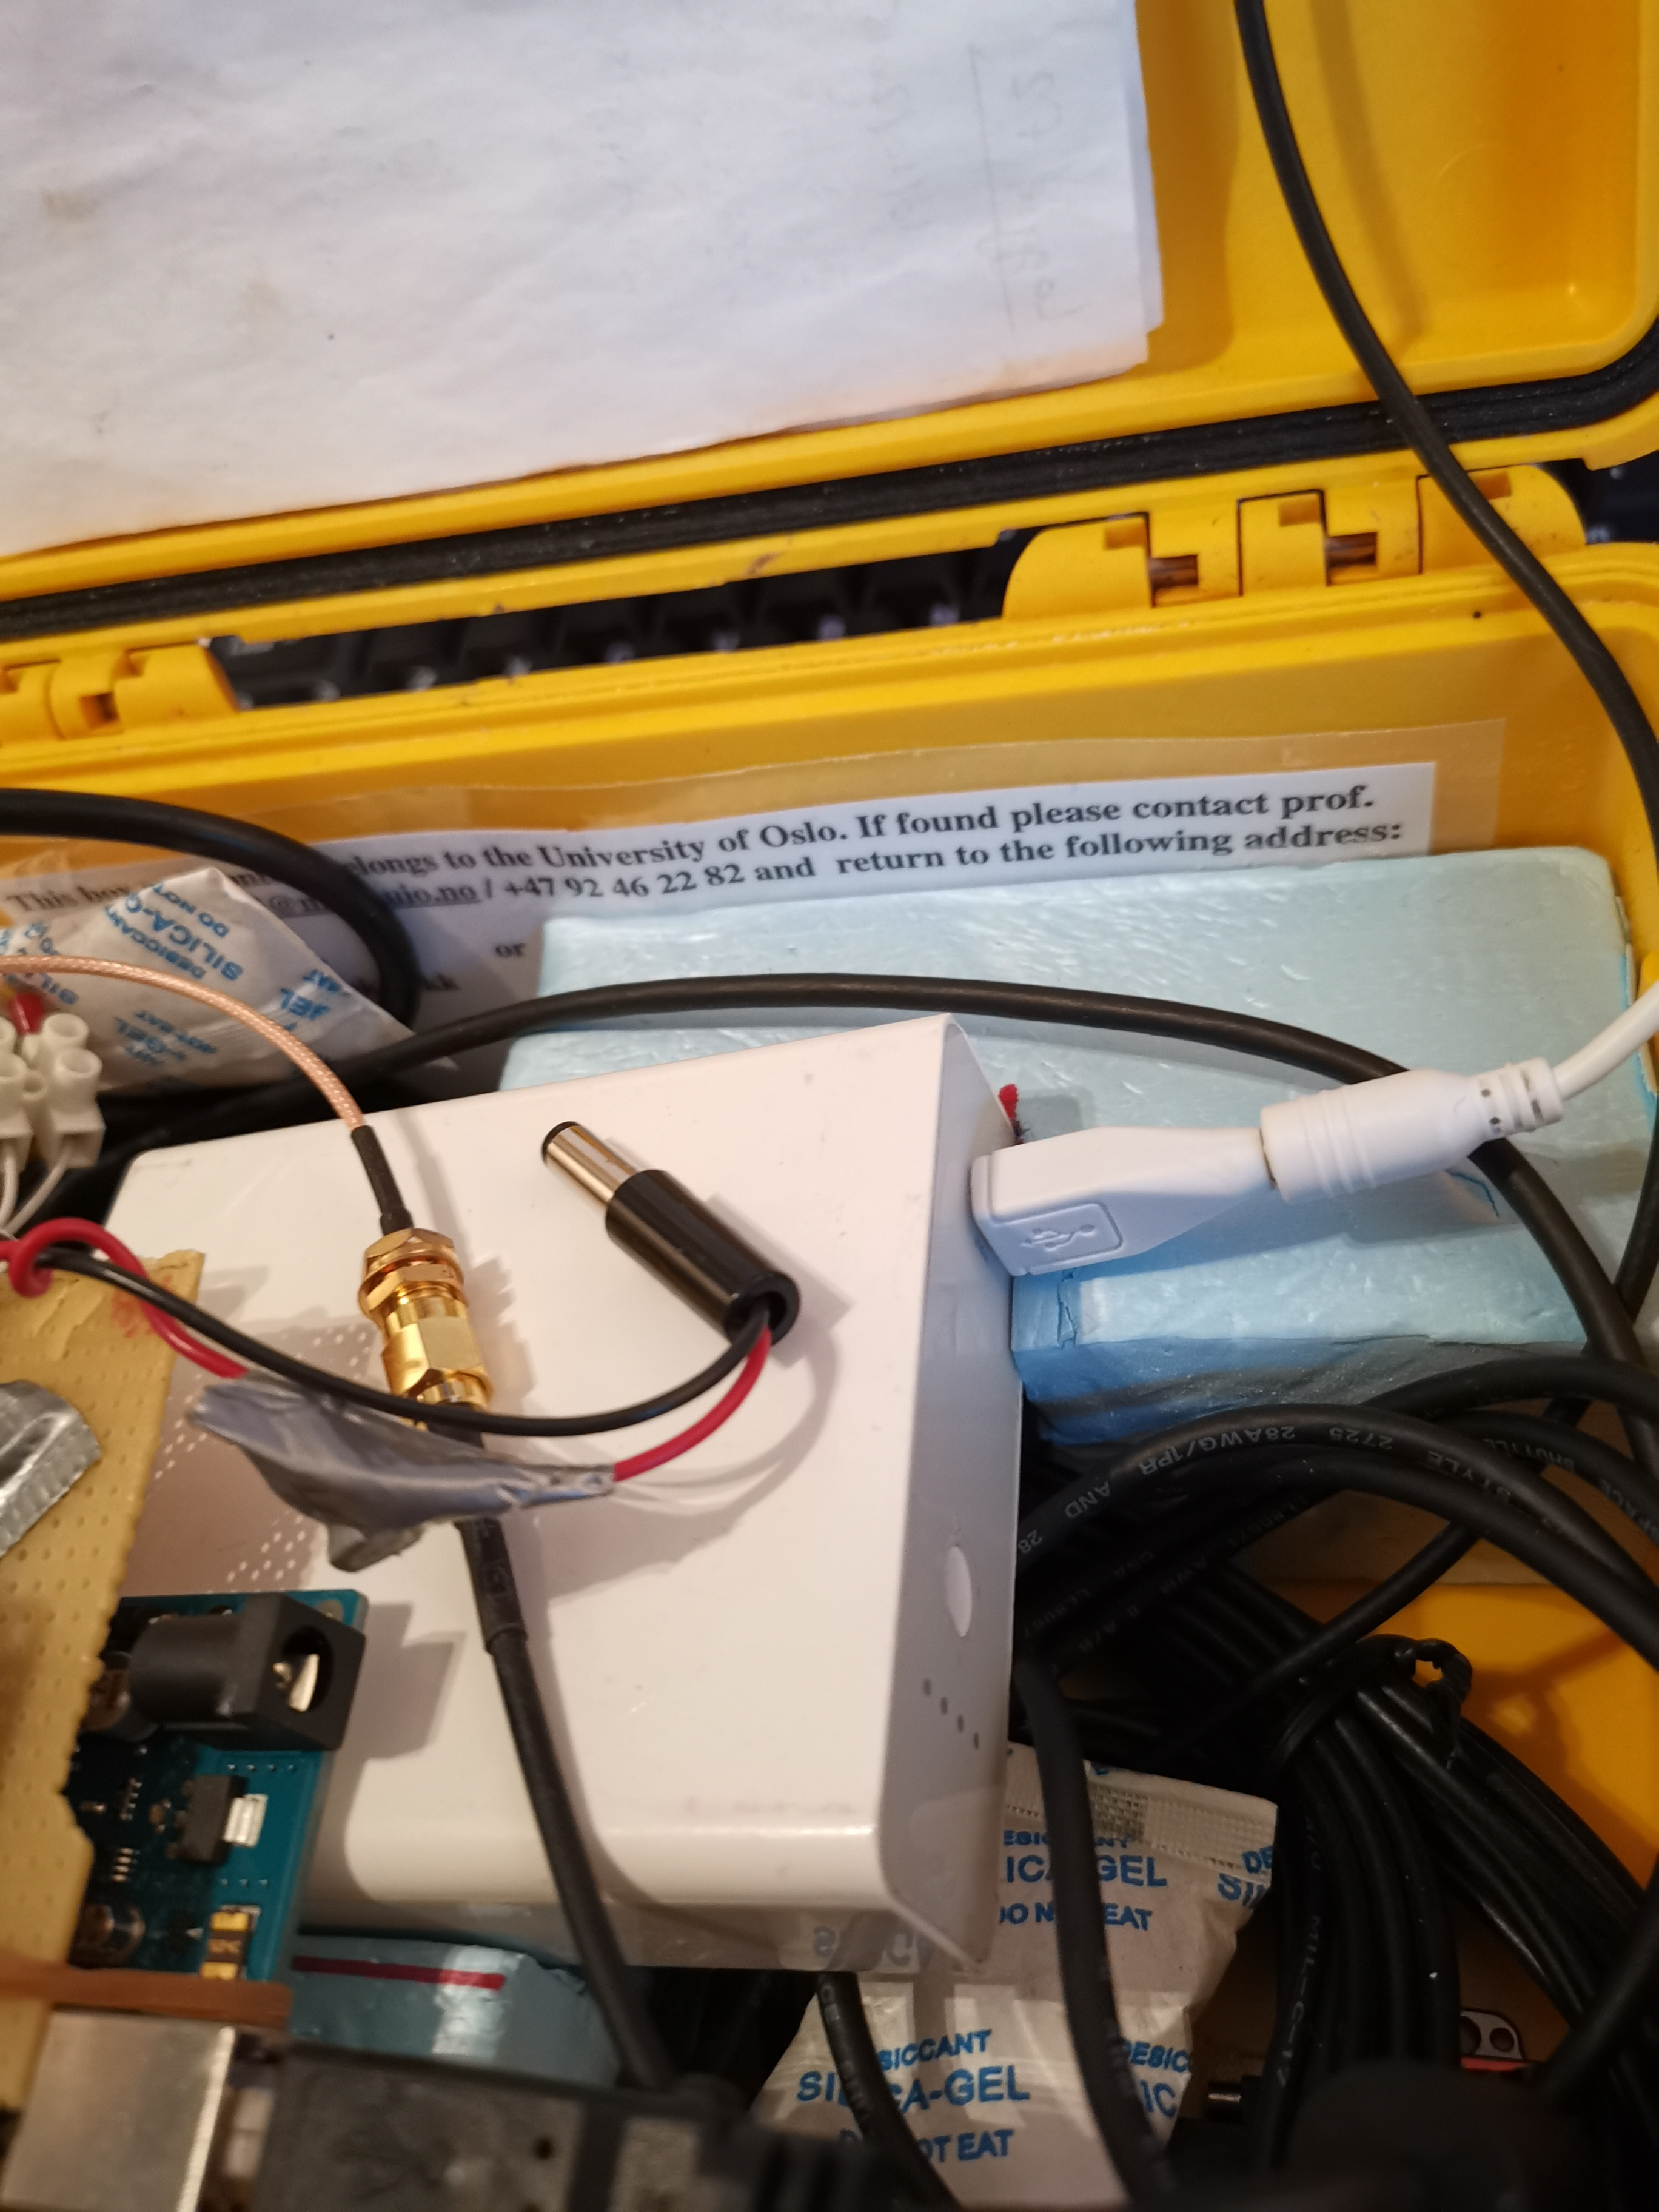
\includegraphics[width=.8\textwidth]{Figures/battery_lift_to_charge}
  \caption{The battery undergoing charging. You do not need to lift the whole battery out of the instrument to recharge, just tilt it. Blue LEDs indicate charge level.}
  \end{center}
  \end{figure}

  \begin{figure}
  \begin{center}
  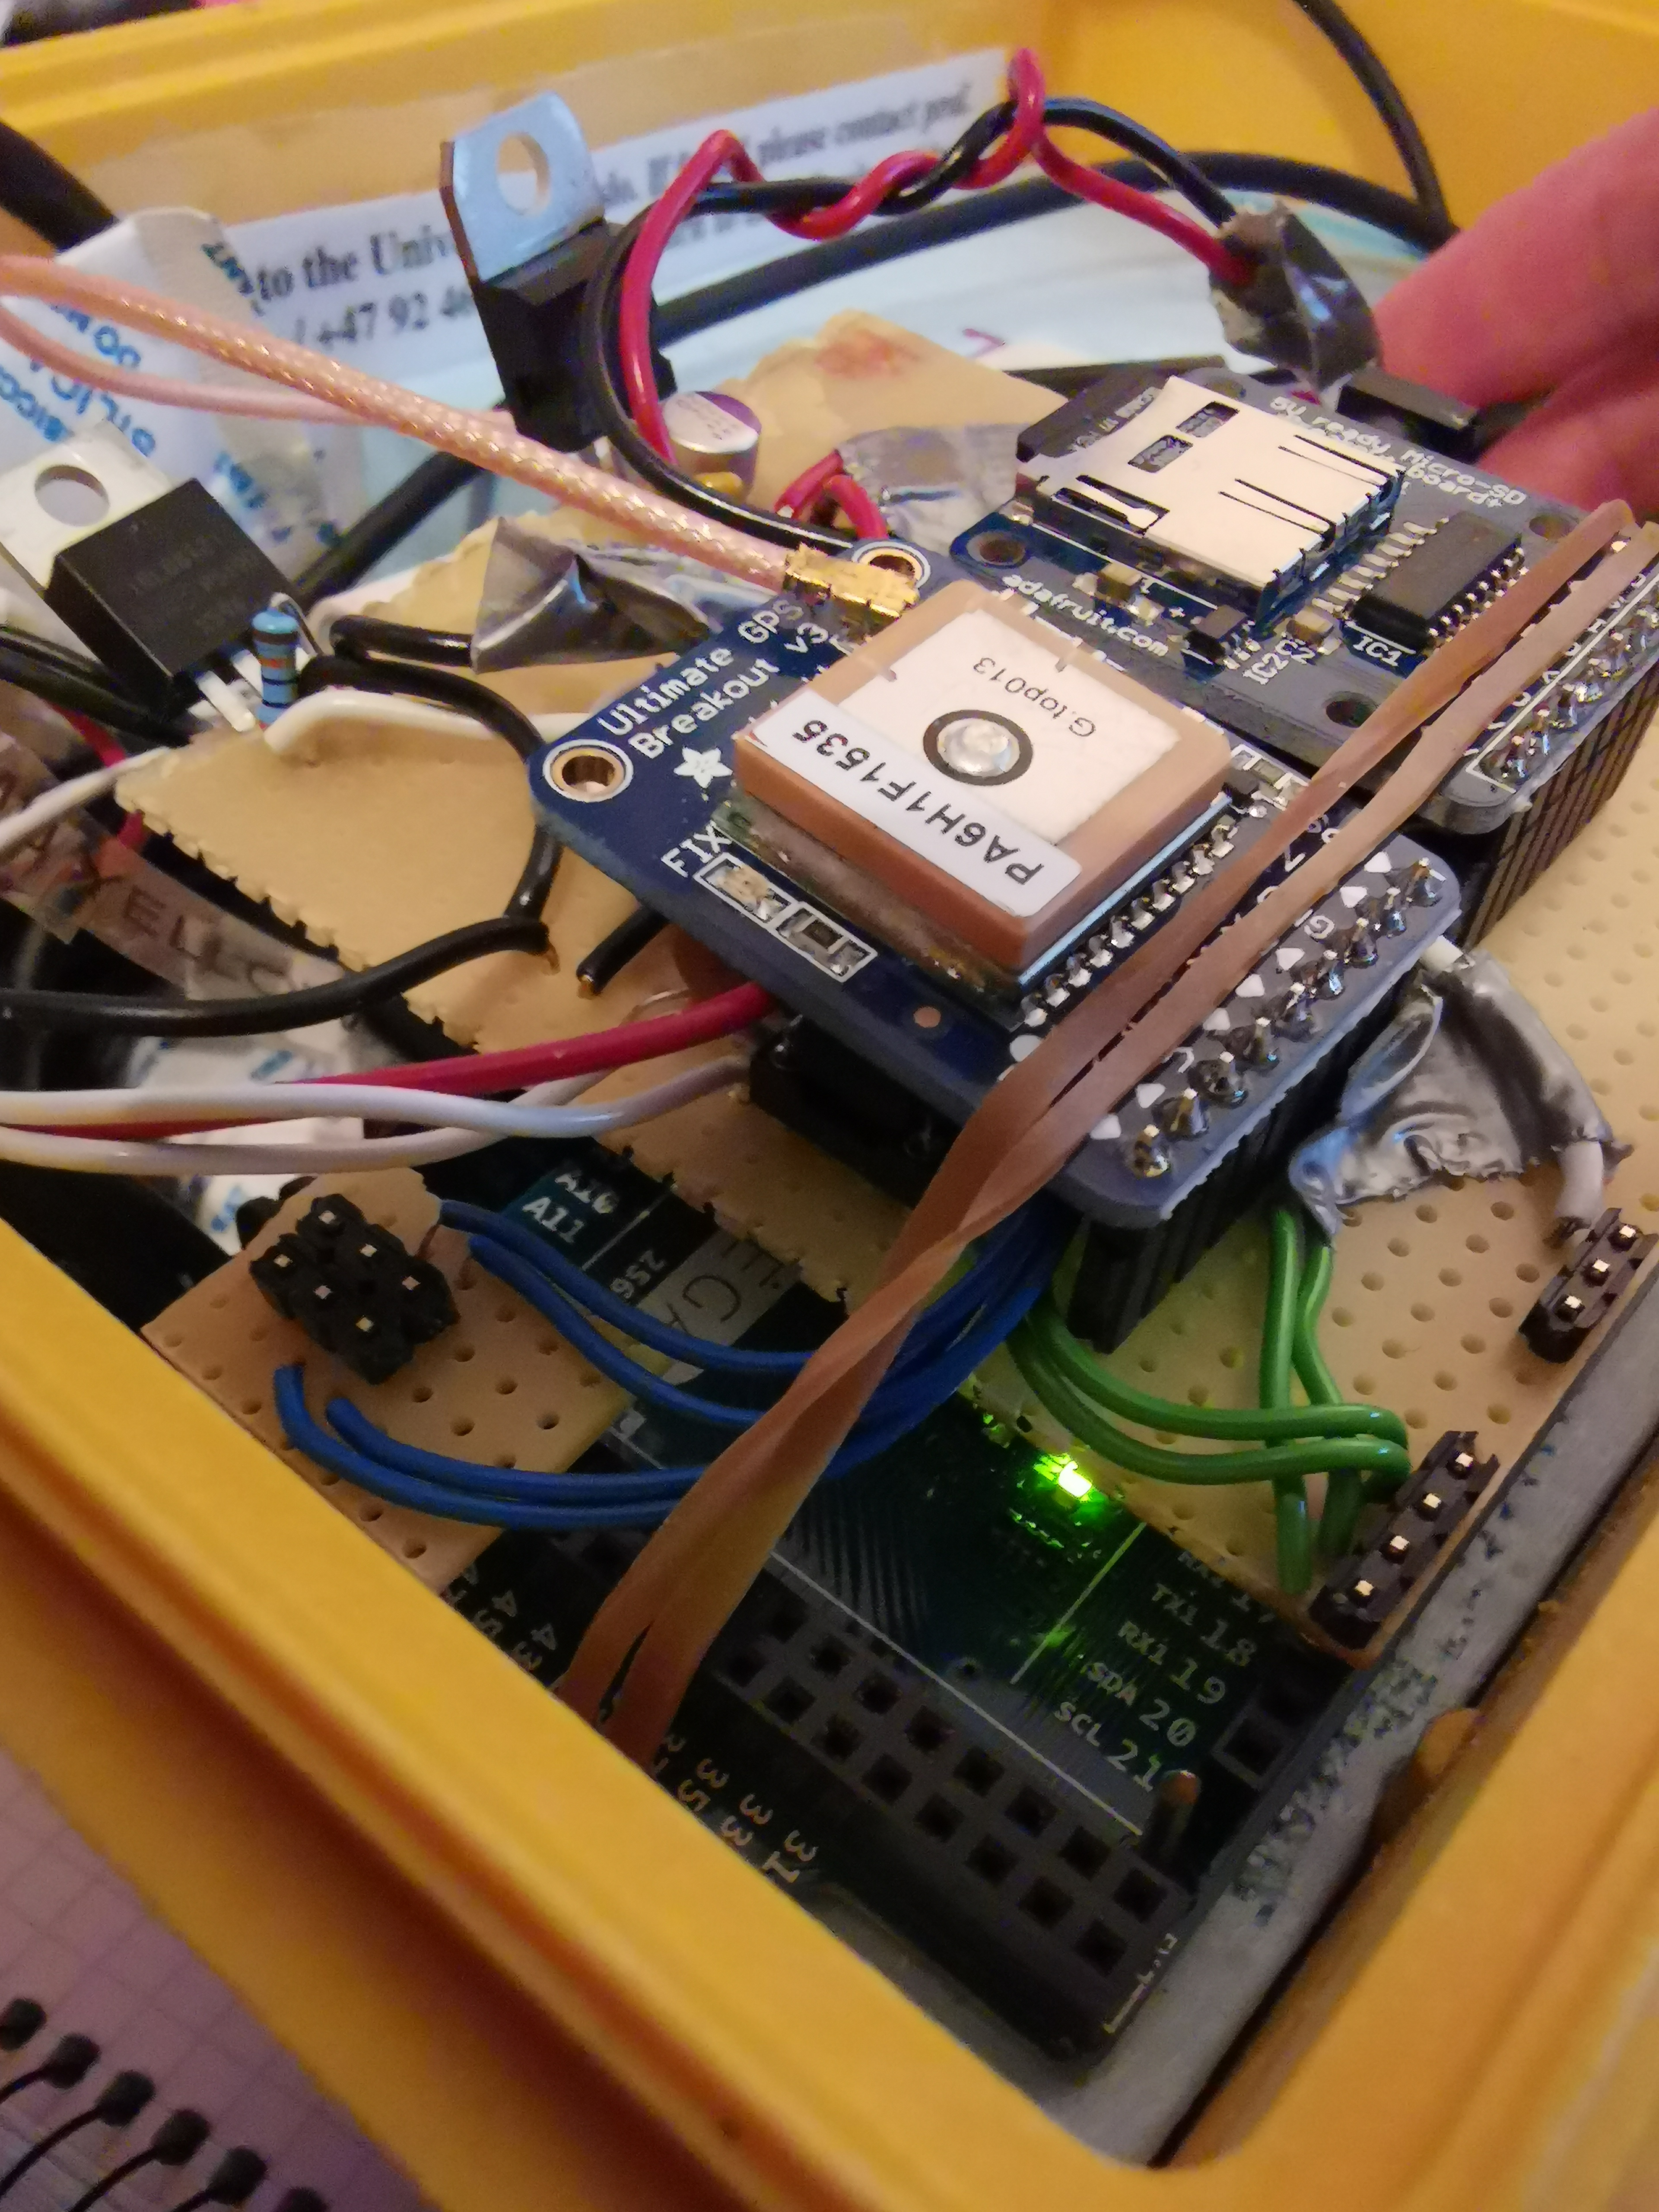
\includegraphics[width=.8\textwidth]{Figures/Arduino_LED}
  \caption{The location of the Arduino green LED (slightly hidden under the PCB).}
  \end{center}
  \end{figure}

\newpage

\section{Starting sequence}

A healthy starting sequence is visible in the video under Figures/video\_starting\_sequence . It shows, following pressing the button to power on the logger:

\begin{itemize}
  \item blue LED turn on on the power bank,
  \item the arduino green LED turns on,
  \item the SD card blinks once,
  \item the GPS LED blinks once,
  \item the SD card LED starts blinking quickly (not regular pattern),
  \item the GPS LED blinks around 1 time per second when looking for GPS satellites; once a GPS fix is obtained, the GPS blinks once each 10 seconds approximately.
\end{itemize}

\section{Tips and tricks}

\begin{itemize}
  \item Do not clamp cables when closing the Pelican Case (this is especially a risk for the cable to the GPS antenna.
  \item Copy the data from the SD card at the end of each deployment if possible.
  \item It should be ok to copy files from the SD cards from Windows computer, but for best result, I would recommend to perform data copy from a Linux computer.
  \item Do not erase data from the SD cards. There is more than enough space on the SD cards for a couple of weeks of activity. I will clean up the SD cards contents after the end of the deployment.
  \item Apply the "usual" condensation care: do not open outside if it rains / snows, if it is cold outside but dry, open the instrument one last time outside to replace warm humid air from the boat with dry cold outside air.
  \item Never exchange SD cards between instruments!
  \item Careful of electrostatic discharges when the pelican case is open. When touching the PCB / electronics, try to first discharge yourself by touching a large mass of metal inside the boat.
  \item The last 15 mintues of data are lost when turning the instrument off. So, in order to have data over the full time when using 2 instruments shifting which one is active each 12 hours, wait at least 15 minutes after the startup of the replacing instrument to switch off hte "old" instrument.
  \item Points to check in case of failure to get a healthy start: 1) is the small side PCB well inserted? 2) is the GPS antenna small connector well inserted? 3) is the SD card well inserted? 4) is everything connected correctly?
  \item New batteries, fully charged, provide around 20 hours of autonomy in the cold. To get continuous measurements over longer time, switch which logger is in use each 12 hours, recharging the battery of the other instrument inside the boat.
\end{itemize}

In case of problem, contact me at: jean.rblt@gmail.com .

\end{document}
